% questions.tex —— 2011 年·山东卷·理科 · 题目内容片段（无答案）
% 由 tools/generate_projects.py 依来源总账自 2011/2011_数学真题_山东理_试题.md 生成，勿手改（改源 MD 后重跑）

\gkpart{一、选择题}

\begin{question}
\gkti{1}设集合 $M=\{x\mid x^2+x-6<0\}$，$N=\{x\mid 1\leqslant x\leqslant 3\}$，则 $M\cap N=$\mbox{（　　）}

（A）$[1,2)$

（B）$[1,2]$

（C）$(2,3]$

（D）$[2,3]$

\end{question}
\begin{question}
\gkti{2}复数 $z=\dfrac{2-\mathrm i}{2+\mathrm i}$（$\mathrm i$ 为虚数单位）在复平面内对应的点所在的象限为\mbox{（　　）}

（A）第一象限

（B）第二象限

（C）第三象限

（D）第四象限

\end{question}
\begin{question}
\gkti{3}若点 $(a,9)$ 在函数 $y=3^x$ 的图象上，则 $\tan\dfrac{a\pi}{6}$ 的值为\mbox{（　　）}

（A）$0$

（B）$\frac{\sqrt3}{3}$

（C）$1$

（D）$\sqrt3$

\end{question}
\begin{question}
\gkti{4}不等式 $|x-5|+|x+3|\geqslant10$ 的解集是\mbox{（　　）}

（A）$[-5,7]$

（B）$[-4,6]$

（C）$(-\infty,-5]\cup[7,+\infty)$

（D）$(-\infty,-4]\cup[6,+\infty)$

\end{question}
\begin{question}
\gkti{5}对于函数 $y=f(x)$，$x\in\mathbf R$。“$y=|f(x)|$ 的图象关于 $y$ 轴对称”是“$y=f(x)$ 是奇函数”的\mbox{（　　）}

（A）充分而不必要条件

（B）必要而不充分条件

（C）充要条件

（D）既不充分也不必要条件

\end{question}
\begin{question}
\gkti{6}若函数 $f(x)=\sin\omega x$（$\omega>0$）在区间 $\left[0,\dfrac{\pi}{3}\right]$ 上单调递增，在区间 $\left[\dfrac{\pi}{3},\dfrac{\pi}{2}\right]$ 上单调递减，则 $\omega=$\mbox{（　　）}

（A）$3$

（B）$2$

（C）$\frac32$

（D）$\frac23$

\end{question}
\begin{question}
\gkti{7}某产品的广告费用 $x$ 与销售额 $y$ 的统计数据如下表：

\begin{center}
\begin{tabular}{lllll}
\toprule
广告费用 $x$（万元） & 4 & 2 & 3 & 5 \\
\midrule
销售额 $y$（万元） & 49 & 26 & 39 & 54 \\
\bottomrule
\end{tabular}
\end{center}

根据上表可得回归方程 $\hat y=\hat bx+\hat a$ 中的 $\hat b$ 为 $9.4$，据此模型预报广告费用为 $6$ 万元时销售额为\mbox{（　　）}

（A）$63.6$ 万元

（B）$65.5$ 万元

（C）$67.7$ 万元

（D）$72.0$ 万元

\end{question}
\begin{question}
\gkti{8}已知双曲线 $\dfrac{x^2}{a^2}-\dfrac{y^2}{b^2}=1$（$a>0$，$b>0$）的两条渐近线均和圆 $C:x^2+y^2-6x+5=0$ 相切，且双曲线的右焦点为圆 $C$ 的圆心，则该双曲线的方程为\mbox{（　　）}

（A）$\frac{x^2}{5}-\frac{y^2}{4}=1$

（B）$\frac{x^2}{4}-\frac{y^2}{5}=1$

（C）$\frac{x^2}{3}-\frac{y^2}{6}=1$

（D）$\frac{x^2}{6}-\frac{y^2}{3}=1$

\Needspace{0.4\textheight}
\end{question}
\begin{question}
\gkti{9}函数 $y=\dfrac x2-2\sin x$ 的图象大致是\mbox{（　　）}

（A）图 A

（B）图 B

（C）图 C

（D）图 D
\nopagebreak[4]
\begin{center}% 2011 年山东卷理科第 9 题：四个选项的函数图象（选项图）。
% 来源 PDF：普通高考/2011/2011山东理.pdf，SHA-256 d0f409fd3fa82b12c210d587c8412d4c446946a201f87d124e2fc17c5a50db16。
% 原页：第 1 页（A3 三栏）第 1 栏下部接第 2 栏上部，书页码 689。
% 重绘依据：原页四图为示意图，纵轴「4」刻度与横轴「2π」刻度的实际比例与 y=x/2-2sin x
%   的取值并不一致（原页纵向压缩），故按 600 dpi 逐像素提取曲线拓扑后重绘，刻度位置照原页：
%   (A) 曲线形如 y=0.31x-1.24cos x（含偶函数项，不关于原点对称，左支与右支不同号）；
%   (B) 曲线形如 y=0.61x-1.84sin x（奇函数，振幅相对一次项小，|x|>4 出图）；
%   (C) 曲线形如 y=0.31x-1.26sin x，与 y=(x/2-2sin x) 同形（零点 ±2.475，极值 x≈±1.32、±4.97、±7.60）；
%   (D) 为奇函数曲线，小极值在 x≈±1.5、大极值在 x≈±6.6，按原页数字化控制点平滑重绘。
%   四图的坐标轴、箭头、刻度「4」「2π」与「O」的位置均照原页，不按比例。
\begin{tikzpicture}[>=stealth, semithick, font=\small, x=0.17cm, y=0.28cm]

  % ================= (A) =================
  \begin{scope}
    \draw[->] (-12.1,0) -- (12.2,0) node[right] {$x$};
    \draw[->] (0,-4.35) -- (0,4.30) node[above] {$y$};
    \draw (-2.4,4) -- (2.4,4);
    \node[left] at (-2.6,4) {$4$};
    \draw (6.283,-0.22) -- (6.283,0.22);
    \node[below] at (6.283,-0.22) {$2\pi$};
    \node at (-2.4,-1.5) {$O$};
    \draw[thick, domain=-10.1:10.1, samples=280]
      plot (\x, {0.31*\x - 1.24*cos(\x r)});
    \node at (-6.4,-6.2) {(A)};
  \end{scope}

  % ================= (B) =================
  \begin{scope}[xshift=7.6cm]
    \draw[->] (-12.1,0) -- (12.2,0) node[right] {$x$};
    \draw[->] (0,-4.35) -- (0,4.30) node[above] {$y$};
    \draw (-2.4,4) -- (2.4,4);
    \node[left] at (-2.6,4) {$4$};
    \draw (6.283,-0.22) -- (6.283,0.22);
    \node[below] at (6.283,-0.22) {$2\pi$};
    \node at (-2.4,-1.5) {$O$};
    \draw[thick, domain=-4.1:4.1, samples=200]
      plot (\x, {0.61*\x - 1.84*sin(\x r)});
    \node at (-6.4,-6.2) {(B)};
  \end{scope}

  % ================= (C) =================
  \begin{scope}[yshift=-6.6cm]
    \draw[->] (-12.1,0) -- (12.2,0) node[right] {$x$};
    \draw[->] (0,-4.35) -- (0,4.30) node[above] {$y$};
    \draw (-2.4,4) -- (2.4,4);
    \node[left] at (-2.6,4) {$4$};
    \draw (6.283,-0.22) -- (6.283,0.22);
    \node[below] at (6.283,-0.22) {$2\pi$};
    \node at (-2.4,-1.5) {$O$};
    \draw[thick, domain=-10.1:10.1, samples=280]
      plot (\x, {0.31*\x - 1.26*sin(\x r)});
    \node at (-6.4,-6.2) {(C)};
  \end{scope}

  % ================= (D) =================
  \begin{scope}[xshift=7.6cm, yshift=-6.6cm]
    \draw[->] (-12.1,0) -- (12.2,0) node[right] {$x$};
    \draw[->] (0,-4.35) -- (0,4.30) node[above] {$y$};
    \draw (-2.4,4) -- (2.4,4);
    \node[left] at (-2.6,4) {$4$};
    \draw (6.283,-0.22) -- (6.283,0.22);
    \node[below] at (6.283,-0.22) {$2\pi$};
    \node at (-2.4,-1.5) {$O$};
    \draw[thick] plot[smooth, tension=0.75] coordinates {
      (-10.08,3.42) (-9.58,2.00) (-8.57,-0.70) (-7.57,-2.38) (-6.55,-2.78)
      (-5.55,-2.20) (-4.53,-1.21) (-3.53,-0.11) (-2.52,0.90) (-1.52,1.30)
      (-0.50,0.70) (0.15,0.20) (0,0) (-0.15,-0.20) (0.50,-0.71)
      (1.52,-1.31) (2.52,-0.90) (3.53,0.11) (4.53,1.21) (5.55,2.20)
      (6.55,2.78) (7.56,2.39) (8.57,0.68) (9.58,-2.02) (10.08,-3.42)};
    \node at (-6.4,-6.2) {(D)};
  \end{scope}

\end{tikzpicture}
\end{center}
\nopagebreak[4]
\end{question}
\begin{question}
\gkti{10}已知 $f(x)$ 是 $\mathbf R$ 上最小正周期为 $2$ 的周期函数，且当 $0\leqslant x<2$ 时，$f(x)=x^3-x$，则函数 $y=f(x)$ 的图象在区间 $[0,6]$ 上与 $x$ 轴的交点的个数为\mbox{（　　）}

（A）$6$

（B）$7$

（C）$8$

（D）$9$

\Needspace{0.4\textheight}
\end{question}
\begin{question}
\gkti{11}如图是长和宽分别相等的两个矩形。给定下列三个命题：① 存在三棱柱，其正（主）视图、俯视图如图；② 存在四棱柱，其正（主）视图、俯视图如图；③ 存在圆柱，其正（主）视图、俯视图如图。其中真命题的个数是\mbox{（　　）}

（A）$3$

（B）$2$

（C）$1$

（D）$0$
\nopagebreak[4]
\begin{center}% 2011 年山东卷理科第 11 题：两个全等矩形的正（主）视图与俯视图。
% 来源 PDF：普通高考/2011/2011山东理.pdf，SHA-256 d0f409fd3fa82b12c210d587c8412d4c446946a201f87d124e2fc17c5a50db16。
% 原页：第 1 页（A3 三栏）第 2 栏中部，书页码 689。
% 重绘依据：照原页——左、右两个同样大小（长宽比约 5:3）的矩形并排，图上无尺寸标注，
%   仅在下方分别标「正（主）视图」「俯视图」；两矩形外框为各自视图的轮廓，不画投影连线。
\begin{tikzpicture}[scale=1.0, semithick]
  \draw (0,0) rectangle (2.4,1.45);
  \node[below] at (1.2,-0.12) {正（主）视图};
  \draw (3.3,0) rectangle (5.7,1.45);
  \node[below] at (4.5,-0.12) {俯视图};
\end{tikzpicture}
\end{center}
\nopagebreak[4]
\end{question}
\begin{question}
\gkti{12}设 $A_1$，$A_2$，$A_3$，$A_4$ 是平面直角坐标系中两两不同的四点，若 $\overrightarrow{A_1A_3}=\lambda\overrightarrow{A_1A_2}$（$\lambda\in\mathbf R$），$\overrightarrow{A_1A_4}=\mu\overrightarrow{A_1A_2}$（$\mu\in\mathbf R$），且 $\dfrac1\lambda+\dfrac1\mu=2$，则称 $A_3$，$A_4$ 调和分割 $A_1$，$A_2$。已知平面上的点 $C$，$D$ 调和分割点 $A$，$B$，则下面说法正确的是\mbox{（　　）}

（A）$C$ 可能是线段 $AB$ 的中点

（B）$D$ 可能是线段 $AB$ 的中点

（C）$C$，$D$ 可能同时在线段 $AB$ 上

（D）$C$，$D$ 不可能同时在线段 $AB$ 的延长线上

\end{question}
\gkpart{二、填空题}

\Needspace{0.4\textheight}
\begin{question}
\gkti{13}执行如图所示的程序框图，输入 $l=2$，$m=3$，$n=5$，则输出的 $y$ 的值是 $\underline{\qquad}$。
\nopagebreak[4]
\begin{center}% 2011 年山东卷理科第 13 题：程序框图。
% 来源 PDF：普通高考/2011/2011山东理.pdf，SHA-256 d0f409fd3fa82b12c210d587c8412d4c446946a201f87d124e2fc17c5a50db16。
% 原页：第 1 页（A3 三栏）第 2 栏下部，书页码 689。
% 重绘依据：照原页——自上而下「开始」→ 平行四边形「输入非负整数 l, m, n」→
%   菱形「l^2+m^2+n^2=0?」：「是」向左下到矩形「y=105」，「否」向下到矩形「y=70l+21m+15n」；
%   再由菱形「y>105?」判断：「是」向右到矩形「y=y-105」并回折上行，汇入「y>105?」上方的竖线；
%   「否」向下经平行四边形「输出 y」到「结束」。y=105 支路的连线向右汇入「输出 y」上方的竖线。
\begin{tikzpicture}[>=stealth, semithick, font=\small]
  \node[draw, rounded corners=0.12cm, minimum width=1.2cm, minimum height=0.5cm] (start) at (0,0) {开始};
  \node[draw, trapezium, trapezium left angle=72, trapezium right angle=108,
        minimum width=3.5cm, minimum height=0.55cm] (input) at (0,-1.15) {输入非负整数 $l$，$m$，$n$};
  \node[draw, diamond, aspect=1.7, minimum width=3.0cm, minimum height=0.95cm] (test1) at (0,-2.55) {$l^2+m^2+n^2=0$};
  \node[draw, minimum width=1.5cm, minimum height=0.55cm] (y105) at (-3.5,-4.15) {$y=105$};
  \node[draw, minimum width=3.4cm, minimum height=0.55cm] (yval) at (0,-4.15) {$y=70l+21m+15n$};
  \node[draw, diamond, aspect=1.7, minimum width=3.0cm, minimum height=0.95cm] (test2) at (0,-5.85) {$y>105$};
  \node[draw, minimum width=2.2cm, minimum height=0.55cm] (dec) at (4.0,-5.85) {$y=y-105$};
  \node[draw, trapezium, trapezium left angle=72, trapezium right angle=108,
        minimum width=1.8cm, minimum height=0.55cm] (out) at (0,-7.3) {输出 $y$};
  \node[draw, rounded corners=0.12cm, minimum width=1.2cm, minimum height=0.5cm] (stop) at (0,-8.4) {结束};
  % 主干
  \draw[->] (start.south) -- (input.north);
  \draw[->] (input.south) -- (test1.north);
  \draw[->] (test1.east) -| (yval.north) node[pos=0.25, right] {否};
  \draw[->] (yval.south) -- (test2.north);
  \draw[->] (test2.south) -- (out.north) node[midway, right] {否};
  \draw[->] (out.south) -- (stop.north);
  % 「是」支路：左侧 y=105，向下汇入「输出 y」上方的竖线
  \draw[->] (test1.west) -| (y105.north) node[pos=0.25, above] {是};
  \draw (y105.south) -- (y105.south |- out.north) -- (out.north);
  % 回环：y=y-105 向左汇入「y>105?」上方竖线
  \draw[->] (test2.east) -- (dec.west) node[midway, above] {是};
  \draw (dec.north) -- (4.0,-4.75) -- (0,-4.75);
\end{tikzpicture}
\end{center}
\nopagebreak[4]
\end{question}
\begin{question}
\gkti{14}若 $\left(x-\dfrac{\sqrt a}{x^2}\right)^6$ 展开式的常数项为 $60$，则常数 $a$ 的值为 $\underline{\qquad}$。

\end{question}
\begin{question}
\gkti{15}设函数 $f(x)=\dfrac{x}{x+2}$（$x>0$），观察：
\nopagebreak[4]
\[f_1(x)=f(x)=\frac{x}{x+2},\]
\nopagebreak[4]
\[f_2(x)=f(f_1(x))=\frac{x}{3x+4},\]
\nopagebreak[4]
\[f_3(x)=f(f_2(x))=\frac{x}{7x+8},\]
\nopagebreak[4]
\[f_4(x)=f(f_3(x))=\frac{x}{15x+16},\]
\nopagebreak[4]
\[\cdots\]
根据以上事实，由归纳推理可得：当 $n\in\mathbf N^*$ 且 $n\geqslant2$ 时，$f_n(x)=f(f_{n-1}(x))=$ $\underline{\qquad}$。

\end{question}
\begin{question}
\gkti{16}已知函数 $f(x)=\log_ax+x-b$（$a>0$，且 $a\neq1$）。当 $2<a<3<b<4$ 时，函数 $f(x)$ 的零点 $x_0\in(n,n+1)$，$n\in\mathbf N^*$，则 $n=$ $\underline{\qquad}$。

\end{question}
\gkpart{三、解答题}

\begin{question}
\gkti{17}在 $\triangle ABC$ 中，内角 $A$，$B$，$C$ 的对边分别为 $a$，$b$，$c$，已知 $\dfrac{\cos A-2\cos C}{\cos B}=\dfrac{2c-a}{b}$。

（1） 求 $\dfrac{\sin C}{\sin A}$ 的值；

（2） 若 $\cos B=\dfrac14$，$b=2$，求 $\triangle ABC$ 的面积 $S$。

\end{question}
\begin{question}
\gkti{18}红队队员甲、乙、丙与蓝队队员 $A$、$B$、$C$ 进行围棋比赛，甲对 $A$、乙对 $B$、丙对 $C$ 各一盘。已知甲胜 $A$、乙胜 $B$、丙胜 $C$ 的概率分别为 $0.6$，$0.5$，$0.5$，假设各盘比赛结果相互独立。

（1） 求红队至少两名队员获胜的概率；

（2） 用 $\xi$ 表示红队队员获胜的总盘数，求 $\xi$ 的分布列和数学期望 $E\xi$。

\Needspace{0.4\textheight}
\end{question}
\begin{question}
\gkti{19}在如图所示的几何体中，四边形 $ABCD$ 为平行四边形，$\angle ACB=90^\circ$，$EA\perp$ 平面 $ABCD$，$EF\parallel AB$，$FG\parallel BC$，$EG\parallel AC$，$AB=2EF$。

（1） 若 $M$ 是线段 $AD$ 的中点，求证：$GM\parallel$ 平面 $ABFE$；

（2） 若 $AC=BC=2AE$，求二面角 $A-BF-C$ 的大小。
\nopagebreak[4]
\begin{center}% 2011 年山东卷理科第 19 题：多面体 ABCD-EFG，AB = 2EF，EF∥AB，FG∥BC，EG∥AC，EA⊥平面 ABCD。
% 来源 PDF：普通高考/2011/2011山东理.pdf，SHA-256 d0f409fd3fa82b12c210d587c8412d4c446946a201f87d124e2fc17c5a50db16。
% 原页：第 2 页（A3 三栏）第 1 栏上部，书页码 690。
% 重绘依据：照原页作斜二测示意（AC = BC = 2AE）。经核实该多面体共有 7 个面：
%   底面 ABCD（平行四边形），面 ABFE（等腰梯形，AB∥EF 且 AB=2EF），面 ADE（三角形），
%   面 BCFG（四边形，FG∥BC），面 CDG（三角形），面 DEG（三角形），面 EFG（三角形）。
%   可见棱（实线）：BC、CD、CG、DE、DG、EF、EG、FB、FG；
%   被遮棱（虚线）：AB、AD、AE；另按原页用虚线画出底面对角线 AC（标出 ∠ACB=90°）与线段 GM（M 为 AD 中点）。
%   拓扑与原页一致，不按比例。
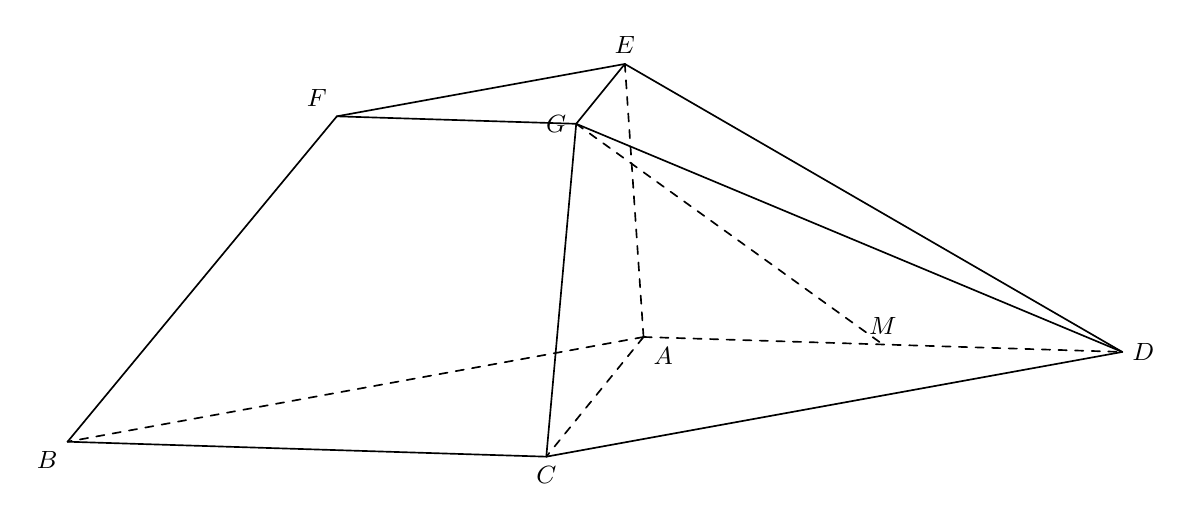
\begin{tikzpicture}[scale=0.95, >=stealth, semithick, font=\small,
  line cap=round]
  \coordinate (B) at (3.60,4.50);
  \coordinate (C) at (10.00,4.30);
  \coordinate (A) at (11.30,5.90);
  \coordinate (D) at (17.70,5.70);
  \coordinate (E) at (11.05,9.55);
  \coordinate (F) at (7.20,8.85);
  \coordinate (G) at (10.40,8.75);
  \coordinate (M) at (14.50,5.80);
  % 可见棱
  \draw (B) -- (C) -- (D);
  \draw (C) -- (G);
  \draw (D) -- (E);
  \draw (D) -- (G);
  \draw (E) -- (F);
  \draw (E) -- (G);
  \draw (F) -- (B);
  \draw (F) -- (G);
  % 被遮棱
  \draw[dashed] (A) -- (B);
  \draw[dashed] (A) -- (D);
  \draw[dashed] (A) -- (E);
  % 底面对角线 AC（原页用虚线画出，以显示 ∠ACB = 90°）
  \draw[dashed] (A) -- (C);
  % 线段 GM（M 为 AD 的中点）
  \draw[dashed] (G) -- (M);
  % 顶点标注
  \node[above] at (E) {$E$};
  \node[above left] at (F) {$F$};
  \node[left] at (G) {$G$};
  \node[below left] at (B) {$B$};
  \node[below] at (C) {$C$};
  \node[below right] at (A) {$A$};
  \node[right] at (D) {$D$};
  \node[above] at (M) {$M$};
\end{tikzpicture}
\end{center}
\nopagebreak[4]
\end{question}
\begin{question}
\gkti{20}等比数列 $\{a_n\}$ 中，$a_1$，$a_2$，$a_3$ 分别是下表第一、二、三行中的某一个数，且 $a_1$，$a_2$，$a_3$ 中的任何两个数不在下表的同一列。

\begin{center}
\begin{tabular}{llll}
\toprule
 & 第一列 & 第二列 & 第三列 \\
\midrule
第一行 & 3 & 2 & 10 \\
第二行 & 6 & 4 & 14 \\
第三行 & 9 & 8 & 18 \\
\bottomrule
\end{tabular}
\end{center}

（1） 求数列 $\{a_n\}$ 的通项公式；

（2） 若数列 $\{b_n\}$ 满足：$b_n=a_n+(-1)^n\ln a_n$，求数列 $\{b_n\}$ 的前 $n$ 项和 $S_n$。

\Needspace{0.4\textheight}
\end{question}
\begin{question}
\gkti{21}某企业拟建造如图所示的容器（不计厚度，长度单位：米），其中容器的中间为圆柱形，左右两端均为半球形，按照设计要求容器的容积为 $\dfrac{80\pi}{3}$ 立方米，且 $l\geqslant2r$。假设该容器的建造费用仅与其表面积有关。已知圆柱形部分每平方米建造费用为 $3$ 千元，半球形部分每平方米建造费用为 $c$（$c>3$）千元。设该容器的建造费用为 $y$ 千元。

（1） 写出 $y$ 关于 $r$ 的函数表达式，并求该函数的定义域；

（2） 求该容器的建造费用最小时的 $r$。
\nopagebreak[4]
\begin{center}% 2011 年山东卷理科第 21 题：圆柱两端各接一个半球形的容器。
% 来源 PDF：普通高考/2011/2011山东理.pdf，SHA-256 d0f409fd3fa82b12c210d587c8412d4c446946a201f87d124e2fc17c5a50db16。
% 原页：第 2 页（A3 三栏）第 2 栏中部，书页码 690。
% 重绘依据：照原页——中间圆柱（长 l，半径 r），左右两端各为半径 r 的半球；
%   两端各画一条竖直虚线（直径，上下各标 r）与一条水平虚线（半径，标 r）；
%   两端的交线圆画成椭圆：靠外的一半实线、靠里的一半虚线（照原页）；
%   顶部用双箭头标出圆柱长 l，箭头两端各有一条竖直短线。不按比例。
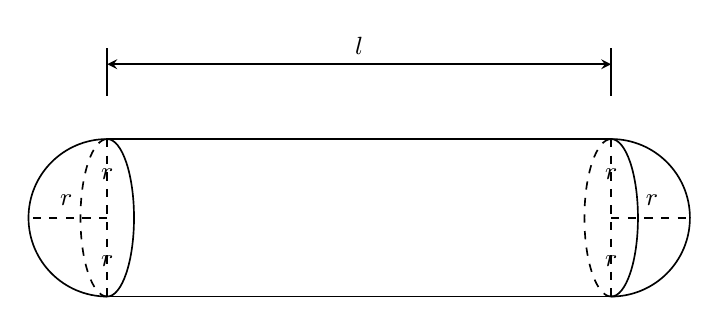
\begin{tikzpicture}[>=stealth, semithick, font=\small, x=1cm, y=1cm]
  \def\r{1.0}
  \def\L{6.4}
  \def\rx{0.34}
  % 圆柱母线
  \draw (0,\r) -- (\L,\r);
  \draw (0,-\r) -- (\L,-\r);
  % 两端半球的外轮廓
  \draw (0,\r) arc (90:270:\r);
  \draw (\L,-\r) arc (-90:90:\r);
  % 左端交线圆：左半实线、右半虚线
  \draw (0,\r) arc (90:-90:{\rx} and {\r});
  \draw[dashed] (0,-\r) arc (-90:-270:{\rx} and {\r});
  % 右端交线圆：左半实线、右半虚线
  \draw (\L,\r) arc (90:-90:{\rx} and {\r});
  \draw[dashed] (\L,-\r) arc (-90:-270:{\rx} and {\r});
  % 左端半径与直径
  \draw[dashed] (0,\r) -- (0,-\r);
  \draw[dashed] (0,0) -- (-\r,0);
  \node at (0,{0.55*\r}) {$r$};
  \node at (0,{-0.55*\r}) {$r$};
  \node at ({-0.52*\r},{0.22*\r}) {$r$};
  % 右端半径与直径
  \draw[dashed] (\L,\r) -- (\L,-\r);
  \draw[dashed] (\L,0) -- ({\L+\r},0);
  \node at (\L,{0.55*\r}) {$r$};
  \node at (\L,{-0.55*\r}) {$r$};
  \node at ({\L+0.52*\r},{0.22*\r}) {$r$};
  % 顶部标注 l
  \draw (\L,{\r+0.55}) -- (\L,{\r+1.15});
  \draw (0,{\r+0.55}) -- (0,{\r+1.15});
  \draw[<->] (0,{\r+0.95}) -- (\L,{\r+0.95});
  \node[above] at ({0.5*\L},{\r+0.95}) {$l$};
\end{tikzpicture}
\end{center}
\nopagebreak[4]
\end{question}
\begin{question}
\gkti{22}已知动直线 $l$ 与椭圆 $C:\dfrac{x^2}{3}+\dfrac{y^2}{2}=1$ 交于 $P(x_1,y_1)$，$Q(x_2,y_2)$ 两不同点，且 $\triangle OPQ$ 的面积 $S_{\triangle OPQ}=\dfrac{\sqrt6}{2}$，其中 $O$ 为坐标原点。

（1） 证明：$x_1^2+x_2^2$ 和 $y_1^2+y_2^2$ 均为定值；

（2） 设线段 $PQ$ 的中点为 $M$，求 $|OM|\cdot|PQ|$ 的最大值；

（3） 椭圆 $C$ 上是否存在三点 $D$，$E$，$G$，使得 $S_{\triangle ODE}=S_{\triangle ODG}=S_{\triangle OEG}=\dfrac{\sqrt6}{2}$？若存在，判断 $\triangle DEG$ 的形状；若不存在，请说明理由。

\end{question}